% answers.tex —— 1988 年·广东卷·文史类 · 参考答案与详细解析片段
% 由 tools/generate_projects.py 依来源总账自 1988/1988_数学真题_广东文_试题.md + 1988/1988_数学真题_广东文_解析正文.md + 1988/1988_数学真题_广东文_答案要点.md 生成，勿手改（改源 MD 后重跑）


\begin{gktip}
固定源 PDF 第 8—21 页含答案与解答。以下按题号规范化转录并统一数学记号；第 3 题和第 24 小题的图形依据固定源重绘为 TikZ。
\end{gktip}

\begin{answer}
\gksolhead{1}{}

\textbf{题目}：

第一卷满分 50 分，共有 25 个选择题。每题都给出代号为 A、B、C、D 的四个结论，其中只有一个结论正确。每题选对得 2 分，不选、选错或者选出的代号超过一个，一律得 0 分。

（1） 在等比数列 $\{a_n\}$ 中，已知 $a_7=6$，$a_9=9$，那么 $a_5=$\mbox{（　　）}

（A）$3$　　（B）$4$　　（C）$\dfrac32$　　（D）$2$

\Needspace{5\baselineskip}
（2） 指数方程

\nopagebreak[4]
\[
2+3^{x-1}=9^{x-\frac12}
\]

的解是\mbox{（　　）}

（A）$0$　　（B）$1$　　（C）$2$　　（D）$\dfrac12$

（3） 直线 $3x-2y=6$ 在 $y$ 轴上的截距是\mbox{（　　）}

（A）$3$　　（B）$-3$　　（C）$2$　　（D）$\dfrac32$

\Needspace{5\baselineskip}
（4） 设

\nopagebreak[4]
\[
P=\left\{x\mathrel{}\middle|\mathrel{}x=\sin\frac{m\pi}{6},\ m\in\mathbb N\right\},\qquad
Q=\left\{x\mathrel{}\middle|\mathrel{}x=\sin\frac{n\pi}{12},\ n\in\mathbb N\right\}.
\]

那么，关于集合 $P$ 和 $Q$ 有\mbox{（　　）}

（A）$P\supset Q$　　（B）$P\subset Q$

（C）$P=Q$　　（D）$P\cap Q=\varnothing$

（5） 用 $1\text{、}2\text{、}3\text{、}4\text{、}5$ 这五个数字，组成没有重复数字的五位数，那么在这些五位数中，是偶数的总共有\mbox{（　　）}

（A）$24$ 个　　（B）$48$ 个　　（C）$60$ 个　　（D）$72$ 个

\Needspace{5\baselineskip}
（6） 当 $\alpha$ 是第二象限的角时，

\nopagebreak[4]
\[
\frac{2\operatorname{tg}\alpha}{\sqrt{\operatorname{sec}^2\alpha-1}}
-\frac{\sqrt{1+\operatorname{tg}^2\alpha}}{\operatorname{sec}\alpha}=
\]

\mbox{（　　）}

（A）$3$　　（B）$1$　　（C）$-1$　　（D）$-3$

（7） 如果 $\operatorname{tg}A+\operatorname{ctg}A=m$，那么 $\sin2A=$\mbox{（　　）}

（A）$\dfrac1m$　　（B）$\dfrac1{m^2}$　　（C）$2m$　　（D）$\dfrac2m$

（8） 设 $a\text{、}b$ 是异面直线，那么\mbox{（　　）}

（A）必然存在唯一的一个平面同时平行于直线 $a$ 和直线 $b$

（B）必然存在唯一的一个平面同时垂直于直线 $a$ 和 $b$

（C）过直线 $a$ 存在唯一的一个平面垂直于直线 $b$

（D）过直线 $a$ 存在唯一的一个平面平行于直线 $b$

\Needspace{5\baselineskip}
（9） 当 $a\ne0$ 时，方程

\nopagebreak[4]
\[
x^2+y^2+ax-ay=0
\]

所表示的图形\mbox{（　　）}

（A）关于 $x$ 轴对称　　（B）关于 $y$ 轴对称

（C）关于直线 $y+x=0$ 对称　　（D）关于直线 $y-x=0$ 对称

\Needspace{5\baselineskip}
（10） 设 $\theta$ 是第四象限的角，那么方程

\nopagebreak[4]
\[
(\sin\theta)x^2+y^2=\sin2\theta
\]

所表示的曲线是\mbox{（　　）}

（A）焦点在 $x$ 轴上的双曲线　　（B）焦点在 $y$ 轴上的双曲线

（C）焦点在 $x$ 轴上的椭圆　　（D）焦点在 $y$ 轴上的椭圆

\Needspace{5\baselineskip}
（11） 抛物线

\nopagebreak[4]
\[
y^2=4x-2
\]

的准线的方程是\mbox{（　　）}

（A）$x=\dfrac14$　　（B）$x=-\dfrac12$　　（C）$x=0$　　（D）$x=-1$

（12） 过抛物线 $y^2=4x$ 的焦点，作直线与此抛物线相交于两点 $P$ 和 $Q$，那么线段 $PQ$ 中点的轨迹方程是\mbox{（　　）}

（A）$y^2=2x-1$　　（B）$y^2=-2x+1$

（C）$y^2=2x-2$　　（D）$y^2=-2x+2$

\Needspace{5\baselineskip}
（13） 函数

\nopagebreak[4]
\[
y=\sqrt{x-2}+1\qquad(x\ge2)
\]

的反函数是\mbox{（　　）}

（A）$y=2-(x-1)^2\ (x\ge1)$　　（B）$y=2+(x-1)^2\ (x\ge1)$

（C）$y=2-(x-1)^2\ (x\ge2)$　　（D）$y=2+(x-1)^2\ (x\ge2)$

（14） 如果奇函数 $f(x)$ 在 $(0,+\infty)$ 上是增函数，那么 $f(x)$ 在 $(-\infty,0)$ 上\mbox{（　　）}

（A）必定是减函数　　（B）必定是增函数

（C）既可能是减函数也可能是增函数　　（D）不一定具有单调性

（15） 已知正三棱台上下底面的边长分别是 $3\,\mathrm{cm}$ 和 $6\,\mathrm{cm}$，斜高是 $\sqrt3\,\mathrm{cm}$，那么侧面和底面所成的二面角等于\mbox{（　　）}

（A）$\dfrac\pi6$　　（B）$\dfrac\pi4$　　（C）$\dfrac\pi3$　　（D）$\dfrac{5\pi}{12}$

（16） “平面 $\alpha$ 内有无穷多条直线都和直线 $l$ 平行”是“$l\parallel\alpha$”的\mbox{（　　）}

（A）充分而不必要的条件　　（B）必要而不充分的条件

（C）必要且充分的条件　　（D）既不充分又不必要的条件

\Needspace{5\baselineskip}
（17） 函数

\nopagebreak[4]
\[
f(x)=2+2x-x^2\qquad(x\in\mathbb R)
\]

的值域是\mbox{（　　）}

（A）$(-\infty,1)$　　（B）$(-\infty,1]$

（C）$(-\infty,3)$　　（D）$(-\infty,3]$

（18） 下列函数中，在区间 $(-\infty,+\infty)$ 上是减函数的只有\mbox{（　　）}

（A）$y=x^{1/3}$　　（B）$y=-\left(\dfrac13\right)^x$

（C）$y=3^x+\left(\dfrac13\right)^x$　　（D）$y=-3^x$

\Needspace{5\baselineskip}
（19） 与不等式

\nopagebreak[4]
\[
\frac{x-3}{2-x}\ge0
\]

同解的不等式是\mbox{（　　）}

（A）$(x-3)(2-x)\ge0$　　（B）$(x-3)(2-x)>0$

（C）$\dfrac{2-x}{x-3}\ge0$　　（D）$\lg(x-2)\le0$

\Needspace{5\baselineskip}
（20）　

\nopagebreak[4]
\[
\operatorname{tg}10^\circ\operatorname{tg}20^\circ
+\sqrt3\left(\operatorname{tg}10^\circ+\operatorname{tg}20^\circ\right)=
\]

（A）$\dfrac1{\sqrt3}$　　（B）$1$　　（C）$\sqrt3$　　（D）$\sqrt6$

（21） 函数值 $\operatorname{tg}224^\circ\text{、}\sin136^\circ\text{、}\cos310^\circ$ 的大小关系是\mbox{（　　）}

（A）$\operatorname{tg}224^\circ<\sin136^\circ<\cos310^\circ$

（B）$\sin136^\circ<\cos310^\circ<\operatorname{tg}224^\circ$

（C）$\cos310^\circ<\sin136^\circ<\operatorname{tg}224^\circ$

（D）$\cos310^\circ<\operatorname{tg}224^\circ<\sin136^\circ$

\Needspace{5\baselineskip}
（22） 函数

\nopagebreak[4]
\[
y=\frac{2+\cos x}{2-\cos x}\qquad(x\in\mathbb R)
\]

的最大值是\mbox{（　　）}

（A）$\dfrac53$　　（B）$\dfrac52$　　（C）$3$　　（D）$5$

\Needspace{5\baselineskip}
（23） 曲线

\nopagebreak[4]
\[
y=\sqrt{2x-x^2}
\]

与直线 $y=k(x-2)+2$ 有两个交点时，实数 $k$ 的取值范围是\mbox{（　　）}

（A）$\left(\dfrac34,1\right]$　　（B）$\left(\dfrac34,+\infty\right)$

（C）$(1,+\infty)$　　（D）$\left[1,\dfrac54\right)$

（24） 已知函数 $y=f(x)$ 的图象如下。
\nopagebreak[4]
\begin{center}% 1988 年广东卷文史类第一卷第 24 小题：固定源中的折线图
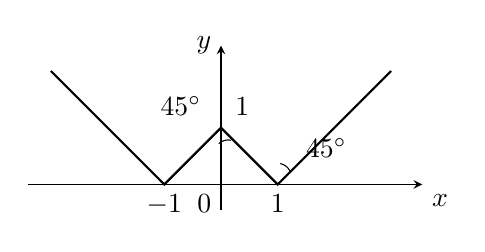
\begin{tikzpicture}[scale=0.72,>=stealth]
  \draw[->] (-3.4,0)--(3.55,0) node[below right] {$x$};
  \draw[->] (0,-0.45)--(0,2.45) node[left] {$y$};
  \draw[thick] (-3.0,2)--(-1,0)--(0,1)--(1,0)--(3.0,2);
  \draw (0.18,0.78) arc (78:132:0.25);
  \draw (1.22,0.23) arc (25:78:0.25);
  \node[above right] at (0.08,1.05) {$1$};
  \node[below left] at (0,0) {$0$};
  \node[below] at (-1,0) {$-1$};
  \node[below] at (1,0) {$1$};
  \node[above left] at (-0.18,1.05) {$45^\circ$};
  \node[above right] at (1.33,0.30) {$45^\circ$};
\end{tikzpicture}
\end{center}
\nopagebreak[4]
那么 $f(x)=$\mbox{（　　）}

（A）$\sqrt{x^2-2x+1}$　　（B）$\sqrt{x^2-2|x|+1}$

（C）$|x^2-1|$　　（D）$x^2-2|x|+1$

\Needspace{5\baselineskip}
（25） 设点 $A(-2,\sqrt3)$，$F$ 为椭圆

\nopagebreak[4]
\[
\frac{x^2}{16}+\frac{y^2}{12}=1
\]

的右焦点，点 $M$ 在该椭圆上移动，当 $|AM|+2|MF|$ 取最小值时，点 $M$ 的坐标是\mbox{（　　）}

（A）$(0,2\sqrt3)$　　（B）$(0,-2\sqrt3)$

（C）$(2\sqrt3,\sqrt3)$　　（D）$(-2\sqrt3,\sqrt3)$

\Needspace{4\baselineskip}
\textbf{解析}

\gksubpart{（1）}

\Needspace{5\baselineskip}
设等比数列的公比为 $q$，则

\nopagebreak[4]
\[
q^2=\frac{a_9}{a_7}=\frac96=\frac32.
\]

\Needspace{5\baselineskip}
又 $a_7=a_5q^2$，所以

\nopagebreak[4]
\[
a_5=\frac{a_7}{q^2}=\frac6{3/2}=4.
\]

故选 B。

\gksubpart{（2）}

\Needspace{5\baselineskip}
令 $t=3^{x-1}>0$，则

\nopagebreak[4]
\[
9^{x-\frac12}=3^{2x-1}=3t^2.
\]

\Needspace{5\baselineskip}
原方程化为

\nopagebreak[4]
\[
3t^2-t-2=0
\quad\Longleftrightarrow\quad
(3t+2)(t-1)=0.
\]

因 $t>0$，只能有 $t=1$，故 $x=1$，选 B。

\gksubpart{（3）}

令 $x=0$，由 $3x-2y=6$ 得 $y=-3$，故选 B。

\gksubpart{（4）}

\Needspace{5\baselineskip}
取 $n=2m$，则

\nopagebreak[4]
\[
\sin\frac{m\pi}{6}=\sin\frac{(2m)\pi}{12}.
\]

所以 $P\subset Q$，选 B。

\gksubpart{（5）}

\Needspace{5\baselineskip}
五位偶数的个位只能是 $2$ 或 $4$。个位固定为其中一个数字时，其余四个数字任意排列，共有 $4!=24$ 种；因此总数为

\nopagebreak[4]
\[
2\cdot4!=48.
\]

故选 B。

\gksubpart{（6）}

\Needspace{5\baselineskip}
当 $\alpha$ 在第二象限时，$\operatorname{tg}\alpha<0$、$\operatorname{sec}\alpha<0$，从而

\nopagebreak[4]
\[
\sqrt{\operatorname{sec}^2\alpha-1}
=|\operatorname{tg}\alpha|
=-\operatorname{tg}\alpha,
\]

\nopagebreak[4]
\[
\sqrt{1+\operatorname{tg}^2\alpha}
=|\operatorname{sec}\alpha|
=-\operatorname{sec}\alpha.
\]

\Needspace{5\baselineskip}
故原式为

\nopagebreak[4]
\[
-2-(-1)=-1,
\]

选 C。

\gksubpart{（7）}

\nopagebreak[4]
\[
\operatorname{tg}A+\operatorname{ctg}A
=\frac{\sin^2A+\cos^2A}{\sin A\cos A}
=\frac1{\sin A\cos A}=m.
\]

\Needspace{5\baselineskip}
所以

\nopagebreak[4]
\[
\sin2A=2\sin A\cos A=\frac2m,
\]

故选 D。

\gksubpart{（8）}

在异面直线 $a$ 上任取一点，过该点作直线 $b'$，使 $b'\parallel b$。直线 $a$ 与 $b'$ 相交，因而确定唯一平面；该平面过 $a$ 且平行于 $b$。故选 D。

\gksubpart{（9）}

\Needspace{5\baselineskip}
配方得

\nopagebreak[4]
\[
\left(x+\frac a2\right)^2+\left(y-\frac a2\right)^2=\frac{a^2}{2}.
\]

圆心为 $\left(-\dfrac a2,\dfrac a2\right)$，满足 $y+x=0$，所以圆关于直线 $y+x=0$ 对称，选 C。

\gksubpart{（10）}

\Needspace{5\baselineskip}
第四象限角满足 $\sin\theta<0$、$\cos\theta>0$。又 $\sin2\theta=2\sin\theta\cos\theta<0$。将方程化为

\nopagebreak[4]
\[
(\sin\theta)x^2+y^2=2\sin\theta\cos\theta.
\]

\Needspace{5\baselineskip}
两边同除以 $\sin\theta$，得

\nopagebreak[4]
\[
x^2+\frac{y^2}{\sin\theta}=2\cos\theta.
\]

其中两个二次项系数异号，且实轴沿 $x$ 轴，表示焦点在 $x$ 轴上的双曲线，选 A。

\gksubpart{（11）}

\nopagebreak[4]
\[
y^2=4x-2=4\left(x-\frac12\right).
\]

\Needspace{5\baselineskip}
抛物线顶点为 $\left(\dfrac12,0\right)$，参数 $p=1$，故准线为

\nopagebreak[4]
\[
x=\frac12-1=-\frac12.
\]

选 B。

\gksubpart{（12）}

\Needspace{5\baselineskip}
抛物线 $y^2=4x$ 的焦点为 $(1,0)$。设过焦点的非竖直直线为 $y=t(x-1)$，与抛物线的两个交点横坐标为 $x_1,x_2$。代入得

\nopagebreak[4]
\[
t^2(x-1)^2=4x.
\]

\Needspace{5\baselineskip}
由韦达定理，交点中点 $(X,Y)$ 满足

\nopagebreak[4]
\[
X=1+\frac2{t^2},\qquad Y=\frac2t.
\]

\Needspace{5\baselineskip}
消去 $t$ 得

\nopagebreak[4]
\[
Y^2=2X-2.
\]

竖直焦点弦的中点 $(1,0)$ 也满足该方程，所以轨迹方程为 $y^2=2x-2$，选 C。

\gksubpart{（13）}

\Needspace{5\baselineskip}
令原函数的自变量为 $u$，由

\nopagebreak[4]
\[
y=\sqrt{u-2}+1
\]

\Needspace{5\baselineskip}
得

\nopagebreak[4]
\[
u=(y-1)^2+2.
\]

\Needspace{5\baselineskip}
原函数的值域为 $[1,+\infty)$，交换自变量与因变量，反函数为

\nopagebreak[4]
\[
y=2+(x-1)^2,\qquad x\ge1.
\]

故选 B。

\gksubpart{（14）}

\Needspace{5\baselineskip}
若 $x_1<x_2<0$，则 $-x_1>-x_2>0$。因 $f$ 在正半轴上递增，

\nopagebreak[4]
\[
f(-x_1)>f(-x_2).
\]

利用奇函数性质 $f(x)=-f(-x)$，可得 $f(x_1)<f(x_2)$，所以在负半轴上仍为增函数，选 B。

\gksubpart{（15）}

\Needspace{5\baselineskip}
在垂直于棱的截面内，正三棱台的上、下底面内切圆半径之差为

\nopagebreak[4]
\[
\frac{6\sqrt3}{6}-\frac{3\sqrt3}{6}=\frac{\sqrt3}{2}.
\]

\Needspace{5\baselineskip}
斜高为 $\sqrt3$，所以台高为

\nopagebreak[4]
\[
h=\sqrt{(\sqrt3)^2-\left(\frac{\sqrt3}{2}\right)^2}=\frac32.
\]

\Needspace{5\baselineskip}
侧面与底面所成二面角 $\varphi$ 满足

\nopagebreak[4]
\[
\tan\varphi=\frac{h}{\sqrt3/2}=\sqrt3.
\]

因 $\varphi$ 为锐角，得 $\varphi=\pi/3$，选 C。

\gksubpart{（16）}

若 $l\parallel\alpha$，则在平面 $\alpha$ 内可以作无穷多条直线与 $l$ 平行，所以题述条件是必要条件。反之，若 $l$ 在平面 $\alpha$ 内，平面内也有无穷多条直线与 $l$ 平行，但按直线与平面平行不相交的定义，不能称 $l\parallel\alpha$。故不是充分条件，选 B。

\gksubpart{（17）}

\nopagebreak[4]
\[
f(x)=2+2x-x^2=3-(x-1)^2\le3.
\]

所以值域为 $(-\infty,3]$，选 D。

\gksubpart{（18）}

在全体实数上，$x^{1/3}$ 是增函数，$-\left(\dfrac13\right)^x$ 也是增函数，$3^x+\left(\dfrac13\right)^x$ 先减后增；而 $-3^x$ 是减函数。因此只有 D。

\gksubpart{（19）}

\Needspace{5\baselineskip}
原不等式的定义域为 $x\ne2$。作符号分析得

\nopagebreak[4]
\[
\frac{x-3}{2-x}\ge0
\quad\Longleftrightarrow\quad
2<x\le3.
\]

\Needspace{5\baselineskip}
又

\nopagebreak[4]
\[
\lg(x-2)\le0
\quad\Longleftrightarrow\quad
0<x-2\le1
\quad\Longleftrightarrow\quad
2<x\le3.
\]

故选 D。

\gksubpart{（20）}

\Needspace{5\baselineskip}
由

\nopagebreak[4]
\[
\tan30^\circ
=\frac{\tan10^\circ+\tan20^\circ}
{1-\tan10^\circ\tan20^\circ}
=\frac1{\sqrt3},
\]

\Needspace{5\baselineskip}
得

\nopagebreak[4]
\[
\sqrt3\left(\tan10^\circ+\tan20^\circ\right)
=1-\tan10^\circ\tan20^\circ.
\]

移项可得原式等于 $1$，选 B。

\gksubpart{（21）}

\nopagebreak[4]
\[
\operatorname{tg}224^\circ=\operatorname{tg}44^\circ,\qquad
\sin136^\circ=\sin44^\circ,\qquad
\cos310^\circ=\cos50^\circ.
\]

\Needspace{5\baselineskip}
显然

\nopagebreak[4]
\[
\cos50^\circ<\sin44^\circ<\operatorname{tg}44^\circ,
\]

故选 C。

\gksubpart{（22）}

\Needspace{5\baselineskip}
令 $t=\cos x\in[-1,1]$，则

\nopagebreak[4]
\[
y=\frac{2+t}{2-t}.
\]

\Needspace{5\baselineskip}
该式关于 $t$ 严格递增，故最大值在 $t=1$ 时取得：

\nopagebreak[4]
\[
y_{\max}=\frac{2+1}{2-1}=3.
\]

选 C。

\gksubpart{（23）}

\Needspace{5\baselineskip}
曲线满足

\nopagebreak[4]
\[
y^2=2x-x^2
\quad\Longleftrightarrow\quad
(x-1)^2+y^2=1,\qquad y\ge0,
\]

\Needspace{5\baselineskip}
是上半圆。将直线写成

\nopagebreak[4]
\[
y=k(x-2)+2.
\]

\Needspace{5\baselineskip}
代入圆方程，关于 $x-1$ 的二次方程判别式为 $4k-3$，所以有两个圆交点需要 $k>3/4$。为了使两个交点都在上半圆上，直线不能越过顶点 $(1,1)$ 的临界位置，得到 $k\le1$。因此

\nopagebreak[4]
\[
\frac34<k\le1,
\]

选 A。

\gksubpart{（24）}

\Needspace{5\baselineskip}
固定源图形的折点为 $(-1,0)$、$(0,1)$、$(1,0)$，两侧斜率的绝对值均为 $1$，且关于 $y$ 轴对称。因此

\nopagebreak[4]
\[
f(x)=\bigl||x|-1\bigr|
=\sqrt{x^2-2|x|+1},
\]

选 B。

\gksubpart{（25）}

\Needspace{5\baselineskip}
椭圆的左、右焦点为 $F_1(-2,0)$、$F(2,0)$。设

\nopagebreak[4]
\[
M=(4\cos t,2\sqrt3\sin t).
\]

\Needspace{5\baselineskip}
由参数式直接计算得

\nopagebreak[4]
\[
|MF|=4-2\cos t.
\]

\Needspace{5\baselineskip}
此外

\nopagebreak[4]
\[
|AM|^2
=19+16\cos t+4\cos^2t-12\sin t.
\]

\Needspace{5\baselineskip}
而

\nopagebreak[4]
\[
|AM|^2-(2+4\cos t)^2
=12\left(\frac54-\cos^2t-\sin t\right)\ge0,
\]

\Needspace{5\baselineskip}
因为在 $\cos^2t+\sin^2t=1$ 下，

\nopagebreak[4]
\[
\cos^2t+\sin t\le\frac54.
\]

\Needspace{5\baselineskip}
当 $\cos t=\sqrt3/2$、$\sin t=1/2$ 时取等号，且对应

\nopagebreak[4]
\[
M=(2\sqrt3,\sqrt3).
\]

\Needspace{5\baselineskip}
在 $\cos t<-1/2$ 时，$8-4\cos t>10$；其余情形由上式有

\nopagebreak[4]
\[
|AM|+2|MF|
\ge(2+4\cos t)+2(4-2\cos t)=10.
\]

所以最小值在 $M=(2\sqrt3,\sqrt3)$ 处取得，选 C。

\gkanswer{答案（1）：B}

\gkanswer{答案（2）：B}

\gkanswer{答案（3）：B}

\gkanswer{答案（4）：B}

\gkanswer{答案（5）：B}

\gkanswer{答案（6）：C}

\gkanswer{答案（7）：D}

\gkanswer{答案（8）：D}

\gkanswer{答案（9）：C}

\gkanswer{答案（10）：A}

\gkanswer{答案（11）：B}

\gkanswer{答案（12）：C}

\gkanswer{答案（13）：B}

\gkanswer{答案（14）：B}

\gkanswer{答案（15）：C}

\gkanswer{答案（16）：B}

\gkanswer{答案（17）：D}

\gkanswer{答案（18）：D}

\gkanswer{答案（19）：D}

\gkanswer{答案（20）：B}

\gkanswer{答案（21）：C}

\gkanswer{答案（22）：C}

\gkanswer{答案（23）：A}

\gkanswer{答案（24）：B}

\gkanswer{答案（25）：C}

\end{answer}
\begin{answer}
\gksolhead{2}{}

\textbf{题目}：

第二卷第一题（本题满分 15 分）共有 5 个小题，每小题满分 3 分。每个小题都有用横线表示的空位，请把你认为合适的内容写在横线上的空位里。

（1） 已知点 $A(1,0)$ 和 $B(2,1)$，那么线段 $AB$ 的垂直平分线方程是　　　　。

\Needspace{5\baselineskip}
（2）　

\nopagebreak[4]
\[
\cos10^\circ\cos55^\circ+\cos80^\circ\cos35^\circ
\]

的值等于　　　　。

（3） 函数 $y=|\sin x|$ 的最小正周期是　　　　。

\Needspace{5\baselineskip}
（4） 设复数

\nopagebreak[4]
\[
z=2\left(\cos\frac\pi6+i\sin\frac\pi6\right),
\]

那么，$z$ 的共轭复数 $\overline z$ 的代数形式是　　　　。

\Needspace{5\baselineskip}
（5）　

\nopagebreak[4]
\[
\lim_{n\to\infty}
\frac{1-2+3-4+\cdots+(2n-1)-2n}{n-1}
\]

的值是　　　　。

\Needspace{4\baselineskip}
\textbf{解析}

\gksubpart{（1）}

\Needspace{5\baselineskip}
$AB$ 的中点为 $\left(\dfrac32,\dfrac12\right)$，而 $AB$ 的斜率为 $1$，故垂直平分线斜率为 $-1$。其方程为

\nopagebreak[4]
\[
y-\frac12=-\left(x-\frac32\right),
\qquad\text{\text{即}}\qquad y=-x+2.
\]

\gksubpart{（2）}

\Needspace{5\baselineskip}
利用积化和差公式：

\nopagebreak[4]
\[
\begin{aligned}
&\cos10^\circ\cos55^\circ+\cos80^\circ\cos35^\circ\\
={}&\frac12(\cos45^\circ+\cos65^\circ)
+\frac12(\cos45^\circ+\cos115^\circ)\\
={}&\cos45^\circ=\frac{\sqrt2}{2}.
\end{aligned}
\]

\gksubpart{（3）}

\Needspace{5\baselineskip}
因为

\nopagebreak[4]
\[
|\sin(x+\pi)|=|-\sin x|=|\sin x|,
\]

所以 $y=|\sin x|$ 的最小正周期为 $\pi$。

\gksubpart{（4）}

\nopagebreak[4]
\[
z=2\left(\cos\frac\pi6+i\sin\frac\pi6\right)
=\sqrt3+i.
\]

\Needspace{5\baselineskip}
故

\nopagebreak[4]
\[
\overline z=\sqrt3-i.
\]

\gksubpart{（5）}

\Needspace{5\baselineskip}
分子成对相减：

\nopagebreak[4]
\[
1-2+3-4+\cdots+(2n-1)-2n=-n.
\]

\Needspace{5\baselineskip}
所以

\nopagebreak[4]
\[
\lim_{n\to\infty}\frac{-n}{n-1}=-1.
\]

\gkanswer{答案（1）：$y=-x+2$}

\gkanswer{答案（2）：$\dfrac{\sqrt2}{2}$}

\gkanswer{答案（3）：$\pi$}

\gkanswer{答案（4）：$\sqrt3-i$}

\gkanswer{答案（5）：$-1$}

\end{answer}
\begin{answer}
\gksolhead{3}{}

\textbf{题目}：

\Needspace{5\baselineskip}
第二卷第二题（本题满分 13 分）。设复数

\nopagebreak[4]
\[
z=-\sqrt6+\sqrt2i,
\]

\Needspace{5\baselineskip}
记

\nopagebreak[4]
\[
u=\left(\frac4z\right)^3.
\]

（1） 求 $|u|$ 和 $\arg u$ 的值。

\Needspace{5\baselineskip}
（2） 求实数 $x$ 和 $y$，使

\nopagebreak[4]
\[
\frac{x}{z}+\frac{y}{u}=z+2u.
\]

\Needspace{4\baselineskip}
\textbf{解析}

\gksubpart{（1）}

\nopagebreak[4]
\[
|z|=\sqrt{6+2}=2\sqrt2.
\]

\Needspace{5\baselineskip}
又

\nopagebreak[4]
\[
|u|=\left|\left(\frac4z\right)^3\right|
=\left(\frac4{2\sqrt2}\right)^3
=2\sqrt2.
\]

\Needspace{5\baselineskip}
复数 $z$ 在第二象限，且其辐角主值为 $5\pi/6$。固定源采用 $0\le\arg u<2\pi$ 的主值约定，因此

\nopagebreak[4]
\[
\arg u=-3\cdot\frac{5\pi}{6}+2k\pi=\frac{3\pi}{2}
\]

\Needspace{5\baselineskip}
（取合适的整数 $k$），故

\nopagebreak[4]
\[
|u|=2\sqrt2,\qquad \arg u=\frac{3\pi}{2}.
\]

\gksubpart{（2）}

\Needspace{5\baselineskip}
由上问 $u=-2\sqrt2\,i$，且

\nopagebreak[4]
\[
\frac1z=\frac{-\sqrt6-\sqrt2\,i}{8},
\qquad
\frac1u=\frac{i}{2\sqrt2}.
\]

\Needspace{5\baselineskip}
代入

\nopagebreak[4]
\[
\frac{x}{z}+\frac{y}{u}=z+2u
\]

\Needspace{5\baselineskip}
得

\nopagebreak[4]
\[
\frac{x}{8}(-\sqrt6-\sqrt2\,i)
+\frac{y}{2\sqrt2}i
=-\sqrt6-3\sqrt2\,i.
\]

\Needspace{5\baselineskip}
比较实部和虚部，得到

\nopagebreak[4]
\[
-\frac{\sqrt6}{8}x=-\sqrt6,\qquad
\frac{y}{2\sqrt2}-\frac{\sqrt2}{8}x=-3\sqrt2,
\]

\Needspace{5\baselineskip}
所以

\nopagebreak[4]
\[
x=8,\qquad y=-8.
\]

\gkanswer{答案（1）：$|u|=2\sqrt2$，$\arg u=\dfrac{3\pi}{2}$。}

\gkanswer{答案（2）：$x=8,\ y=-8$。}

\end{answer}
\begin{answer}
\gksolhead{4}{}

\textbf{题目}：

第二卷第三题（本题满分 14 分）。如图，在四棱锥 $P-ABCD$ 中，$PA\perp$ 底面 $ABCD$，$PD\perp DC$，$DC\parallel$ 侧面 $PAB$。
\nopagebreak[4]
\begin{center}% 1988 年广东卷文史类第二卷第二题：四棱锥 P-ABCD
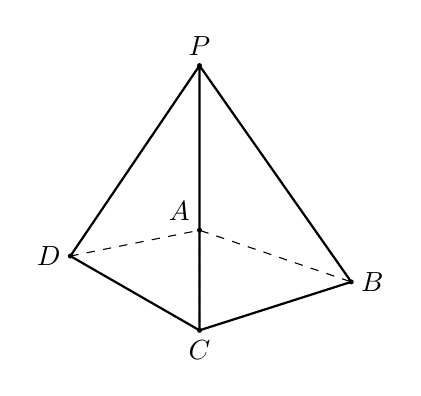
\begin{tikzpicture}[scale=0.82,>=stealth]
  \coordinate (P) at (2.0,4.1);
  \coordinate (D) at (0,1.15);
  \coordinate (C) at (2.0,0);
  \coordinate (B) at (4.35,0.75);
  \coordinate (A) at (2.0,1.55);
  \draw[thick] (P)--(D) (P)--(C) (P)--(B);
  \draw[dashed] (P)--(A);
  \draw[thick] (D)--(C)--(B);
  \draw[dashed] (D)--(A)--(B) (A)--(C);
  \fill (P) circle (1.1pt) node[above] {$P$};
  \fill (A) circle (1.1pt) node[above left] {$A$};
  \fill (B) circle (1.1pt) node[right] {$B$};
  \fill (C) circle (1.1pt) node[below] {$C$};
  \fill (D) circle (1.1pt) node[left] {$D$};
\end{tikzpicture}
\end{center}
\nopagebreak[4]
（1） 求证：$DA\perp AB$。

（2） 又设 $PB=PC$，且 $DC=PA=3\,\mathrm{cm}$，$DA=4\,\mathrm{cm}$，求这个四棱锥的体积。

\Needspace{4\baselineskip}
\textbf{解析}

\gksubpart{（1）}

\Needspace{5\baselineskip}
由 $PA\perp$ 底面，$DA$ 是斜线 $PD$ 在底面上的射影。又 $PD\perp DC$，由三垂线定理的逆定理，

\nopagebreak[4]
\[
DA\perp DC.
\]

\Needspace{5\baselineskip}
因 $DC\parallel$ 平面 $PAB$，且底面 $ABCD$ 与平面 $PAB$ 的交线为 $AB$，故

\nopagebreak[4]
\[
DC\parallel AB.
\]

\Needspace{5\baselineskip}
于是

\nopagebreak[4]
\[
DA\perp AB.
\]

\gksubpart{（2）}

\Needspace{5\baselineskip}
由 $PA\perp$ 底面及第（1）问，三角形 $PAD$、$PDC$、$PAB$ 均为直角三角形。于是

\nopagebreak[4]
\[
PD=\sqrt{PA^2+DA^2}
=\sqrt{3^2+4^2}=5\,\mathrm{cm},
\]

\nopagebreak[4]
\[
PC=\sqrt{PD^2+DC^2}
=\sqrt{5^2+3^2}=\sqrt{34}\,\mathrm{cm}.
\]

\Needspace{5\baselineskip}
由 $PB=PC$ 及 $PA\perp AB$，

\nopagebreak[4]
\[
AB=\sqrt{PB^2-PA^2}
=\sqrt{34-9}=5\,\mathrm{cm}.
\]

\Needspace{5\baselineskip}
底面是以 $DA$ 为高的直角梯形，且 $DC\parallel AB$，所以

\nopagebreak[4]
\[
S_{ABCD}
=\frac12(AB+DC)\,DA
=\frac12(5+3)\cdot4=16\,\mathrm{cm}^2.
\]

\Needspace{5\baselineskip}
四棱锥的高为 $PA=3\,\mathrm{cm}$，故

\nopagebreak[4]
\[
V=\frac13S_{ABCD}\cdot PA
=\frac13\cdot16\cdot3
=16\,\mathrm{cm}^3.
\]

\gkanswer{答案（1）：$DA\perp AB$。}

\gkanswer{答案（2）：$16\,\mathrm{cm}^3$。}

\end{answer}
\begin{answer}
\gksolhead{5}{}

\textbf{题目}：

\Needspace{5\baselineskip}
第二卷第四题（本题满分 14 分）。设数列 $\{a_n\}$ 的前 $n$ 项和

\nopagebreak[4]
\[
S_n=\frac\pi3n^2+c,
\]

式中 $c$ 是常数，$n=1,2,\ldots$。

（1） 如果 $c\ne0$，求证：$\{a_n\}$ 不是等差数列。

\Needspace{5\baselineskip}
（2） 如果 $c=0$，求证：对任意大于 1 的自然数 $n$，和数

\nopagebreak[4]
\[
\cos^2(a_{n-1})+\cos^2(a_n)+\cos^2(a_{n+1})
\]

是一个与 $n$ 无关的常数，并求出这个常数值。

\Needspace{4\baselineskip}
\textbf{解析}

\gksubpart{（1）}

\nopagebreak[4]
\[
a_1=S_1=\frac\pi3+c.
\]

\Needspace{5\baselineskip}
当 $n\ge2$ 时，

\nopagebreak[4]
\[
\begin{aligned}
a_n
&=S_n-S_{n-1}\\
&=\left(\frac\pi3n^2+c\right)
-\left(\frac\pi3(n-1)^2+c\right)\\
&=\frac\pi3(2n-1).
\end{aligned}
\]

\Needspace{5\baselineskip}
因此当 $n\ge3$ 时，

\nopagebreak[4]
\[
a_n-a_{n-1}=\frac{2\pi}{3},
\]

\Needspace{5\baselineskip}
而

\nopagebreak[4]
\[
a_2-a_1=\pi-\left(\frac\pi3+c\right)
=\frac{2\pi}{3}-c.
\]

当 $c\ne0$ 时两者不等，故 $\{a_n\}$ 不是等差数列。

\gksubpart{（2）}

\Needspace{5\baselineskip}
当 $c=0$ 时，上式对 $n=1$ 也成立，即

\nopagebreak[4]
\[
a_n=\frac\pi3(2n-1).
\]

\Needspace{5\baselineskip}
并且

\nopagebreak[4]
\[
a_{n+1}=a_n+\frac{2\pi}{3},\qquad
a_{n-1}=a_n-\frac{2\pi}{3}.
\]

\Needspace{5\baselineskip}
利用

\nopagebreak[4]
\[
\cos\left(a_n-\frac{2\pi}{3}\right)
=-\frac12\cos a_n+\frac{\sqrt3}{2}\sin a_n,
\]

\nopagebreak[4]
\[
\cos\left(a_n+\frac{2\pi}{3}\right)
=-\frac12\cos a_n-\frac{\sqrt3}{2}\sin a_n,
\]

\Needspace{5\baselineskip}
可得

\nopagebreak[4]
\[
\begin{aligned}
&\cos^2a_{n-1}+\cos^2a_n+\cos^2a_{n+1}\\
={}&\left(-\frac12\cos a_n+\frac{\sqrt3}{2}\sin a_n\right)^2
+\cos^2a_n\\
&\quad+\left(-\frac12\cos a_n-\frac{\sqrt3}{2}\sin a_n\right)^2\\
={}&\frac32\left(\cos^2a_n+\sin^2a_n\right)
=\frac32.
\end{aligned}
\]

所以该和与 $n$ 无关，常数值为 $\dfrac32$。

\gkanswer{答案（1）：$\{a_n\}$ 不是等差数列。}

\gkanswer{答案（2）：常数为 $\dfrac32$。}

\end{answer}
\begin{answer}
\gksolhead{6}{}

\textbf{题目}：

\Needspace{5\baselineskip}
第二卷第五题（本题满分 14 分）。设 $k$ 和 $r$ 是实数，且 $r>0$，使得：直线 $y=kx+1$ 既与圆

\nopagebreak[4]
\[
x^2+y^2=r^2
\]

\Needspace{5\baselineskip}
相切，又与双曲线

\nopagebreak[4]
\[
x^2-y^2=r^2
\]

有两个交点。

（1） 求证：$\dfrac1{r^2}-k^2=1$，且 $|k|\ne1$。

（2） 试问：直线 $y=kx+1$ 能否经过双曲线 $x^2-y^2=r^2$ 的焦点？为什么？

\Needspace{4\baselineskip}
\textbf{解析}

\gksubpart{（1）}

\Needspace{5\baselineskip}
直线 $y=kx+1$ 与圆 $x^2+y^2=r^2$ 相切，因此圆心到直线的距离等于半径：

\nopagebreak[4]
\[
\frac{|1|}{\sqrt{1+k^2}}=r.
\]

\Needspace{5\baselineskip}
平方并整理得

\nopagebreak[4]
\[
\frac1{r^2}-k^2=1.
\]

\Needspace{5\baselineskip}
再将 $y=kx+1$ 代入双曲线 $x^2-y^2=r^2$，得

\nopagebreak[4]
\[
(1-k^2)x^2-2kx-(1+r^2)=0.
\]

\Needspace{5\baselineskip}
直线与双曲线有两个交点，故该方程必须是二次方程，从而 $1-k^2\ne0$，即

\nopagebreak[4]
\[
|k|\ne1.
\]

\gksubpart{（2）}

\Needspace{5\baselineskip}
双曲线

\nopagebreak[4]
\[
x^2-y^2=r^2
\]

\Needspace{5\baselineskip}
的焦点为

\nopagebreak[4]
\[
F_1(-\sqrt2\,r,0),\qquad F_2(\sqrt2\,r,0).
\]

\Needspace{5\baselineskip}
若直线经过 $F_1$，则

\nopagebreak[4]
\[
-\sqrt2\,kr+1=0,
\qquad\text{\text{即}}\qquad
\frac1r=\sqrt2\,k.
\]

\Needspace{5\baselineskip}
与第（1）问结论合并，得到

\nopagebreak[4]
\[
(\sqrt2\,k)^2-k^2=1
\quad\Longrightarrow\quad
k^2=1,
\]

这与 $|k|\ne1$ 矛盾。经过 $F_2$ 时同理。因此直线 $y=kx+1$ 不能经过双曲线的任一焦点。

\gkanswer{答案（1）：$\dfrac1{r^2}-k^2=1$，且 $|k|\ne1$。}

\gkanswer{答案（2）：不能经过双曲线的任一焦点。}

\end{answer}